\documentclass{article}
\usepackage[utf8]{inputenc}
\usepackage[left=1.50cm, right=1.50cm, top=1.50cm, bottom=1.50cm]{geometry}
\usepackage{blindtext}
\usepackage{multicol}
\usepackage{graphicx}
\usepackage{listings}
\usepackage{xcolor}

\title{Ecuación general de segundo grado en C}
\author{Gustavo Ramos}
\date{7 de Enero de 2024}

\definecolor{codegreen}{rgb}{0,0.6,0}
\definecolor{codegray}{rgb}{0.5,0.5,0.5}
\definecolor{codepurple}{rgb}{0.58,0,0.82}
\definecolor{backcolour}{rgb}{0.95,0.95,0.92}

\lstdefinestyle{mystyle} {
	backgroundcolor=\color{backcolour},   
	commentstyle=\color{codegreen},
	keywordstyle=\color{magenta},
	numberstyle=\tiny\color{codegray},
	stringstyle=\color{codepurple},
	basicstyle=\ttfamily\footnotesize,
	breakatwhitespace=false,         
	breaklines=true,                 
	captionpos=b,                    
	keepspaces=true,                 
	numbers=left,                    
	numbersep=5pt,                  
	showspaces=false,                
	showstringspaces=false,
	showtabs=false,                  
	tabsize=2
}

\lstset{style=mystyle}

\begin{document}

	\maketitle
	\begin{multicols}{2}

		\section{Resumen}
			La siguiente práctica expone pasos para desarrollar un programa que resuelve la ecuación cuadrática en el lenguaje c

		\section{Introducción }
			"Si lo puedes imaginar, lo puedes programar", es la frase que ha motivado a los grandes programadores a
			crear obras de arte que todos hemos usado en nuestro día a día, sobre todo en matemáticas, los lenguajes de
			programación se escribieron para hacer matemáticas numéricas, en esta ocasión usaremos la capacidad del
			lenguaje c para resolver la ecuación de segundo grado, una ecuación muy antigua que dio paso a los números
			imaginarios.

		\section{Marco teórico }
			Primero tenemos que entender el problema, y antes hemos visto como resolver una ecuación de segundo
			grado y las propiedades de sus raíces ayudándonos del determinante, que para una ecuación definida como
			$ax^2+bx+c=0$, su discriminante esta definido como $\Delta=b^2-4ac$

		\subsection{Ecuación "cuadrática" con $a=0$ }
			Si la ecuación tiene como coeficiente cuadrático $a=0$, no es una ecuación cuadrática, sino una lineal
			de la forma: 
			$$bx+c=0$$
			La solución de una ecuación lineal es fácil de calcular y es:
			$$x=-\frac{c}{b}$$

		\subsection{Soluciones generales}
			De manera general, y demostrado anteriormente, las ecuaciones cuadráticas tienen dos soluciones cuyas son:
			$$x_{1,2}=\frac{-b\pm\sqrt{\Delta}}{2a}=\frac{-b\pm\sqrt{b^2-4ac}}{2a},\hspace{0.5cm}a\neq0$$

		\subsection{Soluciones reales}
			Si $\Delta>0$, la raíz seria un numero real, así pues, tenemos:
			$$x_{1,2}=\frac{-b\pm\sqrt{\Delta}}{2a}=\frac{-b\pm\sqrt{b^2-4ac}}{2a},\hspace{0.5cm}a\neq0$$

		\subsection{Soluciones imaginarias}
			Si $\Delta<0$, podemos factorizar un $-1$ del determinante y se cumple $-\Delta>0$ y que 
			$\sqrt{-(-\Delta)}=i\sqrt{-\Delta}$, ademas que $\sqrt{-\Delta}\in R$
			así pues, tenemos que las soluciones son:
			$$x_{1,2}=\frac{-b\pm\sqrt{\Delta}}{2a}=\frac{-b}{2a}\pm{i}\frac{\sqrt{-\Delta}}{2a}=\frac{-b}{2a}\pm{i}\frac{\sqrt{b^2-4ac}}{2a},\hspace{0.5cm}a\neq0$$

		\subsection{Solución doble}
			Si $\Delta=0$, solo tenemos una solución, esta solución es doble y es:
			$$x=\frac{-b}{2a},\hspace{0.5cm}a\neq0$$

	\end{multicols}

	\section{Diseño de código }

	\lstinputlisting[language=c]{../main.c}
	\newpage

	\begin{multicols}{2}
		\section{Análisis  de resultados}
			De los cuatro casos obtenidos anteriormente, se asignaron las variables correspondientes para la obtención de cada una de las raíces:\\
			Para una ecuación lineal: 
			\begin{center}
				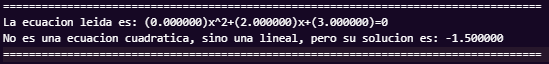
\includegraphics[scale=0.63]{Caso1.png}
			\end{center}
			Para una ecuación con raíces reales:
			\begin{center}
				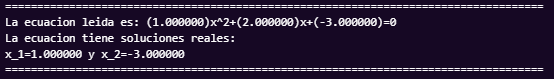
\includegraphics[scale=0.63]{Caso2.png}
			\end{center}
			Para una ecuación con raíces complejas
			\begin{center}
				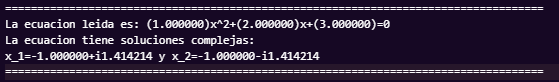
\includegraphics[scale=0.63]{Caso3.png}
			\end{center}
			Para una ecuación con raíz doble
			\begin{center}
				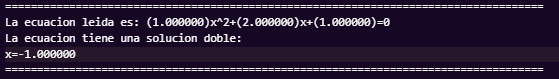
\includegraphics[scale=0.63]{Caso4.png}
			\end{center}

		\section{Conclusiones}
			El código funciona como se esperaría, escribe las soluciones de una manera entendible, el declarar las variables de manera global ahorra muchas lineas.

		\section{Referencias }
			[1] Lehmann C.H (2009). Álgebra. México. Limusa.
	\end{multicols}

\end{document}